\documentclass[a4paper,french,10pt]{article}
\usepackage[utf8]{inputenc}
\usepackage[french]{babel}
\usepackage{graphicx}
\usepackage{float}
\addtolength{\oddsidemargin}{-2,5cm}
\addtolength{\textwidth}{5cm}
\addtolength{\topmargin}{-2,5cm}
\addtolength{\textheight}{4cm}

\title{\textbf{TALN -- Extraction à base de règles\\ \normalsize Extraction automatique de dates de soumission dans un corpus d'appels à contribution}}
\author{Thibaut \textsc{Marmin} \and Clément \textsc{Sipieter}}
\date{31 Mai 2011}

\begin{document}

\maketitle

\emph{Nous avons fait le choix de développer une commande permettant, à partir d'un message texte (par exemple un email et son header), de retourner la liste des dates contenues dans ce dernier. Chacune est couplée à une note de confiance, située entre zéro et un, renseignant sur la fiabilité d'un date à être une date de soumission.}

\section{Utilitaire de séparation}
Un premier utilitaire de pré-traitement à été développé en Java. Il permet, à partir du fichier de corpus complet, d'extraire chaque email et de les exporter dans des fichiers séparés.

Les fichiers générés contiennent l'entête de l'email et le message.

\section{Utilitaire de recherche de dates}
Dans le but de pouvoir réutiliser notre application, nous avons fait le choix de développer une simple commande, prenant en entrée un email avec son entête sous la forme d'une chaine de caractères, et retourne la liste des dates de soumission associées à une note de confiance.

\begin{figure}[H]
\centering
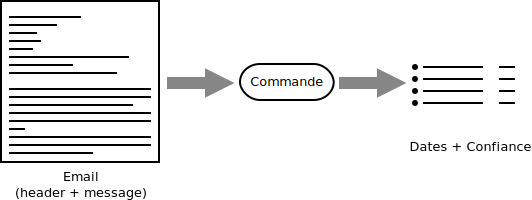
\includegraphics[width=0.6\textwidth]{files/archi}
\caption{Entrée / Sortie de la commande}
\end{figure}

L'application a été développée en Java et utilise notamment les classes fournies par l'API permettant de gérer les dates et les expressions régulières.

\subsection{Traitement}

\subsubsection{Suppression de l'entête}
Le premier traitement effectué est la suppression de l'entête. Ce processus est effectué en supprimant toutes les lignes comprises entre la chaine \og \texttt{From -} \fg{} et la première ligne vide suivante rencontrée.

\subsubsection{Détection des dates}
La détection des dates contenues dans le corps de l'email s'effectue à l'aide d'expressions régulières. Une date pouvant être écrite de nombreuses manières dans un texte, l'expression régulière permettant leurs détections est longue. Nous avons donc fait le choix de la générer à l'aide de la classe \texttt{Date} proposée par l'API Java. Cette méthode nous a permis d'obtenir une recherche de dates dans de multiple formats et langues.

\paragraph*{Expression régulière générée :}

\begin{verbatim}
ici la regexp
\end{verbatim}

La méthode de recherche de dates a été validée par la mise en place de nombreux tests unitaires.

\subsection{Détection des mots clés}
La seconde étape consiste à rechercher dans le message des mots clés pertinents, ayant comme principale caractéristique d'assurer la proximité certaine d'une date de soumission. Pour ce faire, nous avons avons analysé quelques mails afin d'établir une liste de mots clés.

Exemples de mots clés : \texttt{submi / soume / soumi / camera-paper}

A noter que nous avons choisi dans certains cas de ne noter que le stemme afin d'englober plusieurs mots clés.

\subsection{Évaluation des dates}

Notre algorithme de calcul de confiance des dates fonctionne de la manière suivante :

\begin{itemize}
\item L'email est vu comme une droite (chaine de caractères), parcourue de gauche à droite.
\item Cette droite est parsemée de mots clés, de dates, et d'obstacles (représentant certains caractères discriminatoires).
\item Un mot clé va influencer positivement la confiance que l'on a en date. Cette influence diminue avec la distance.
\item Les obstacles représentent certains caractères discriminatoires, faisant ainsi diminuer radicalement leur influence.
\item Une date absorbe totalement l'influence d'un mot clé. La confiance d'une date est déterminée par la somme de toutes les influences qu'elle perçoit.
\end{itemize}

La figure~\ref{fig:representation_email} représente un morceau d'email, contenant quatre mots clés, deux dates et un obstacle. Sous la droite sont représentées les niveaux d'influence des quatre mots clés. Le niveau de confiance représenté en violet est la somme des niveaux d'influence perçus.

\begin{figure}[H]
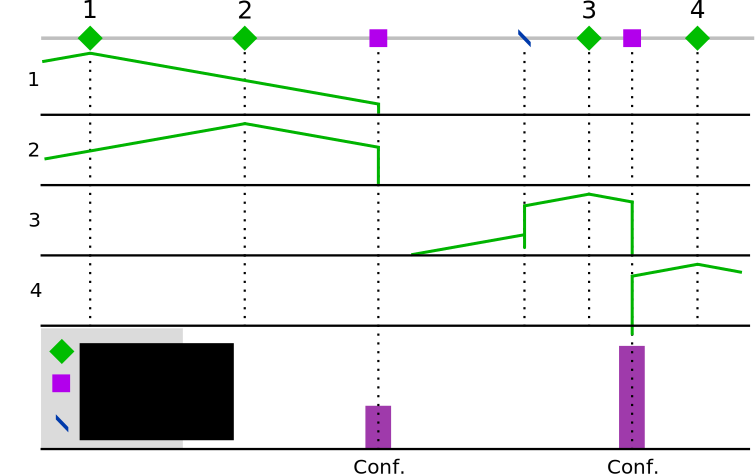
\includegraphics[width=\textwidth]{files/representation_email}
\caption{Représentation schématique d'un email et de l'influence des mots clés.}
\label{fig:representation_email}
\end{figure}


\end{document}
